\section{Background}

% supercomputing
% 超算的网络需求和混合虚拟环境
Supercomputing is high-performance for data-intensive or compute-intensive tasks, e.g. deep learning training and big data processing. To meet the performance demands, supercomputing are generally constructed in a cluster which includes multiple machine instances. So, there are urge demands for network between instances in supercomputing. RDMA is a popular high-performance network in supercomputing. Meanwhile, to utilize the server resources, supercomputing are going cloud, especially hybrid virtual environments.

% Container and VM
% 虚拟机和容器的差异导致虚拟化时的虚拟层的位置通常不同
Virtualization for VMs and containers are in different spaces because of their characteristics. Virtual machines are hardware-level virtualization which need emulate whole virtual hardware environments for guest operation system with hypervisor(Kernel-space) So, applications in VMs is securate due to guest OS isolation, but needs more transform overhead. Containers are OS-level virtualization which isolate anc control the kernel resources, such as network and file system. So, containers have less loss in performance. Containers are managemented by container engeins which are located in user-space for lightweight and portability. So, when virtualization for VMs, the virtual layer is commonly in OS(hypervisor) and is in user-space for containers.

% RDMA: 
% RDMA网卡是控制和数据路径分离, RDMA网卡内部构造
% RDMA网卡数据传输机制,按门铃操作
RDMA(Remote Direct Memory Access) has hardware protocol stack and zero copy technology, so applications can bypass the kernel to read and write remote memory data, without the participation of remote CPU. As a result, RDMA has high throughput, low latency and low CPU load. Applications need to use Verbs interface when using RDMA. In Verbs, as shown in Figure~\ref{fig:rdma-feat}, RDMA is seperate control path and data path. The former is the managemet about RDMA context, mainly including lots of RDMA resources, such as Queue Pairs(QPs), and Memory Reigions(MRs). the operations like ibv\_create\_qp, reg\_mr; The latter is the usage of RDMA context and resources,  which is the data commands like ibv\_post\_send and ibv\_post\_recv. In a RDMA workflow, the communication is based on Queue Pair (QP). The application writes the RDMA work request to the QP, and then ``press''  the RNIC's doorbell register, which is mapped to application when initing context, and the RNIC's hardware processor will execute the work request in the QP to forward data. For applications, the entire operator is in the user space.

\begin{figure}[!ht]
	\centering
	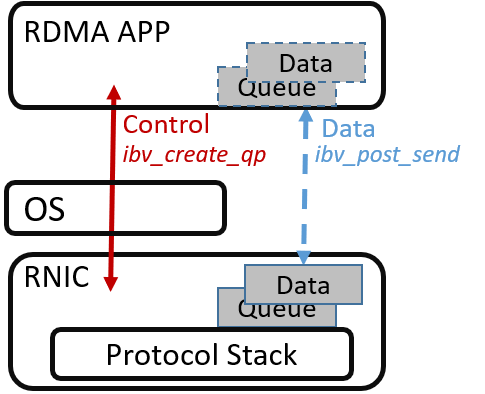
\includegraphics[width=0.6\linewidth]{images/rdma-feat}
	\caption{Native RDMA Feature}
	\label{fig:rdma-feat}
\end{figure}


